\documentclass[10pt]{article}
\usepackage[utf8]{inputenc}
\usepackage[english]{babel}
\usepackage{amsmath}
\usepackage{graphicx}
\usepackage{float}
\usepackage{lipsum}
\usepackage{multicol}
\usepackage{xcolor}
\usepackage{tabularx}
\usepackage{booktabs}
\usepackage{hyperref}
\usepackage{float}
\usepackage{stfloats}
\usepackage{placeins}
\usepackage{wrapfig}
\usepackage{caption}
\usepackage[absolute,overlay]{textpos}
\setlength{\TPHorizModule}{1cm} % Horizontal unit (adjust as needed)
\setlength{\TPVertModule}{1cm}  % Vertical unit (adjust as needed)
\newcolumntype{Y}{>{\centering\arraybackslash}X}
\usepackage[left=2.00cm, right=2.00cm, top=2.00cm, bottom=2.00cm]{geometry}
\usepackage[table,xcdraw]{xcolor}
\title{AN2DL First Homework Report}

\begin{document}
    
    \begin{figure}[H]
        \raggedright
        
\includegraphics[scale=0.4]{polimi.png} \hfill 
\includegraphics[scale=0.3]{airlab.jpeg}
    \end{figure}
    
    \vspace{5mm}
    
    \begin{center}
        % Select between First and Second
        {\Large \textbf{AN2DL - First Homework Report}}\\
        \vspace{2mm}
        % Change with your Team Name
        {\Large \textbf{NeuralDropouts}}\\
        \vspace{2mm}
        % Team Members Information
        {\large Pinar Erbil,}
        {\large Sergio Pardo,}
        {\large Angela Remolina,}
        {\large Matteo Sissa}\\
        \vspace{2mm}
        % Codabench Nicknames
        {perbil,}
        {sergiopardo,}
        {angelaremolina,}
        {matteosissa}\\
        \vspace{2mm}
        % Matriculation Numbers
        {244638,}
        {243066,}
        {242814,}
        {247064}\\
        \vspace{5mm}
        \today
    \end{center}    
    \vspace{5mm}
    
    \begin{multicols}{2}
    
    \section{Introduction}
        
        From healthcare to transportation, AI-powered systems are enhancing efficiency, accuracy, and accessibility in ways previously unimaginable. Technologies like deep learning and deep neural networks have also allowed huge improvements in the computer vision field.
        Medical Image Analysis falls in-between these two areas, it implements cutting edge deep learning models to boost the capability humanity has of studying our body and its composition. This is the context of the present project, which aims to \textbf{classify images of blood cells among 8 possible classes}. 

        
    \section{Problem Analysis}

        Classifying blood cells is a complex task due to the subtle differences among various cell types, which can lead to significant challenges in accurate identification. The analysis of the problem starts with the inspection of the available dataset which is composed of 13759 96x96 RGB, all labeled with an integer value ranging between 0 and 7 to representing the 8 classes of blood cells.
        %respectively Basophil, Eosinophil, Erythroblast, Immature granulocytes, Lymphocyte, Monocyte, Neutrophil, Platelet. 
        The correctness of the labels provided in the original dataset, presumably derived from expert knowledge, was assumed throughout the project.

    
    \section{Method}
        \label{sec:method}
        %To address the classification problem, the following methodology was employed.
        
        \subsection{Data wrangling}
        \label{sec:wrangling}
        First, the dataset was inspected using \textbf{Principal Component Analysis (PCA)}  \cite{jolliffe2016principal} to identify outliers and erroneous data points. In this analysis, it was clear that the points located farther from the origin were identified as outliers. See figure \ref{fig:fig1}.       

        \begin{figure}[H]
        \frame{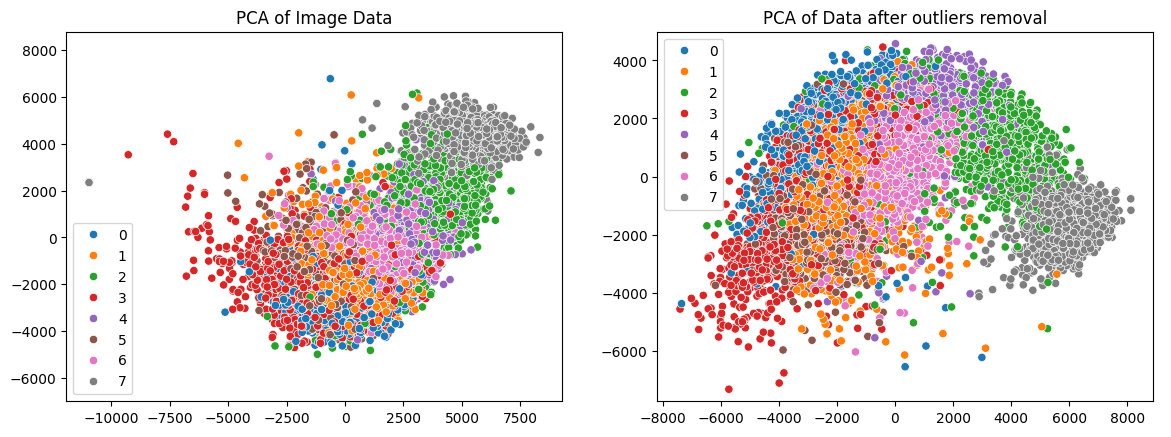
\includegraphics[width=0.9\linewidth]{images/pca.png}}
        \centering
        \caption{PCA before and after outlier removal}
        \label{fig:fig1}
        \end{figure}
        
        Upon examining these points, it becomes evident that the organizers of the competition included several irrelevant samples. Specifically, a total of 200 images of meme 1 and 1600 images of meme 2 were found, amounting to 1800  samples that were deleted from the dataset. % See figure \ref{fig:fig2}

        

        % \begin{figure}[H]
        % \frame{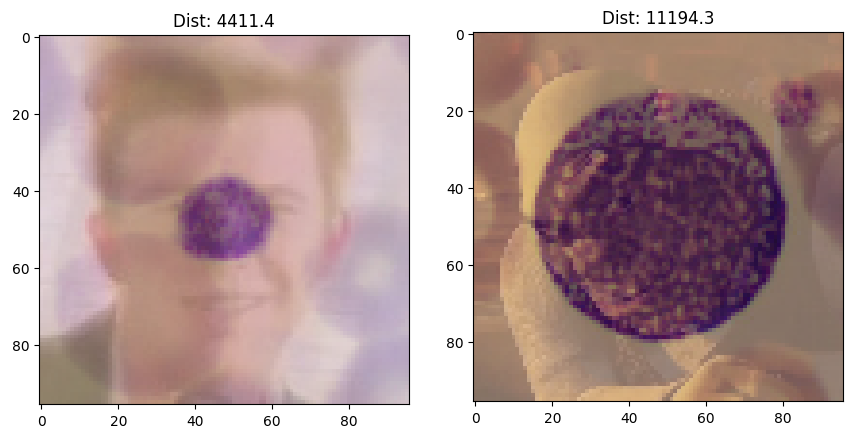
\includegraphics[width=0.6\linewidth]{images/memes.png}}
        % \centering
        % \caption{Memes found in dataset}
        % \label{fig:fig2}
        % \end{figure}

        
        \subsection{Data Augmentation}
        \label{sec:aug}
        \textbf{Augmentation} turned out to be a key step to mitigate overfitting, given the variability in imaging conditions and the limited size of the original dataset.\\
        The first augmentation attempt was trying to highlight key features of the cell like, removing background and showing more clear edges, see \ref{fig:edge}.
        \begin{figure}[H]
        \frame{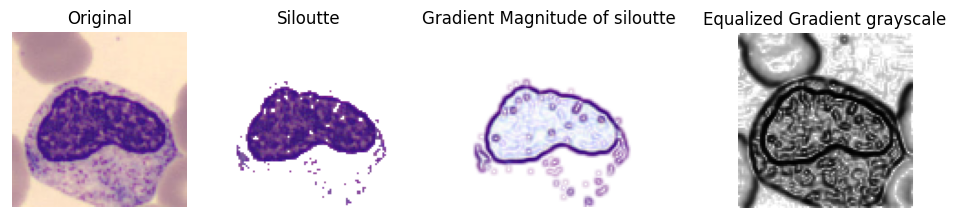
\includegraphics[width=1\linewidth]{images/edge.png}}
        \centering
        \caption{Edge highlighting augmentation}
        \label{fig:edge}
        \end{figure}
        These looks really good to the human eye, but the performance obtained by the model were not good, so this technique was discarded. \\
        The augmentation step of the dataset was thoroughly redesigned, applying more advanced techniques like FourierMix \cite{fouriermix}, and CutMix \cite{cutmix}. See figure \ref{fig:final_aug}
        These augmented samples plus the original one were fed to the model for training. 
        \begin{figure}[H]
        \frame{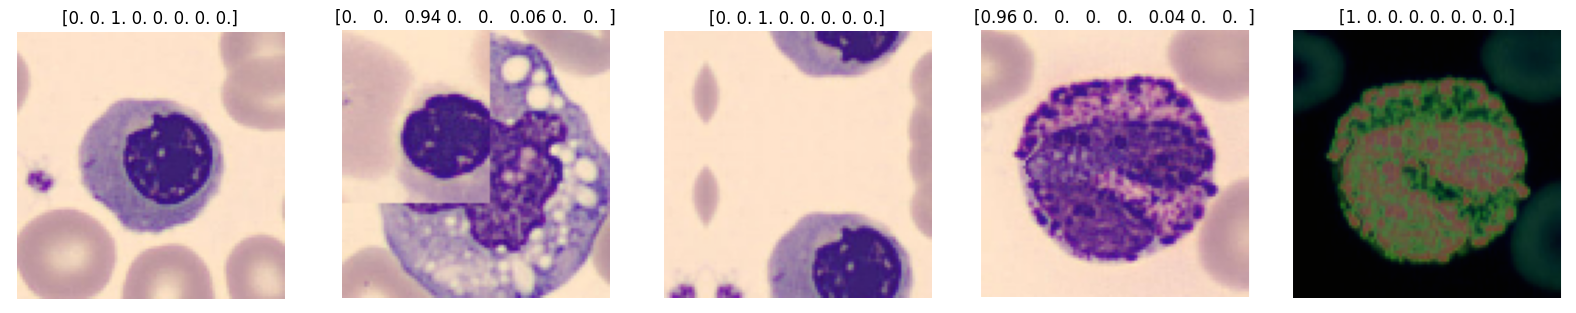
\includegraphics[width=1\linewidth]{images/final_aug.png}}
        \centering
        \caption{FourierMix, CutMix, RandAugment}
        \label{fig:final_aug}
        \end{figure}
        % todo: add specific explination of augmentation in block approach
        
        \subsection{Model design and transfer learning from pretrained model}
        Instead of training a custom model from scratch, \textbf{transfer learning} was applied.
        This approach is advantageous as it exploits the strong feature extraction capabilities of a pre-trained large model that are crucial for distinguishing subtle differences in blood cells with a limited dataset.\\
        ConvNextXLarge \cite{liu2022convnext}, trained on the ImageNet dataset \cite{deng2009imagenet}, was selected to provide the feature extraction network for the classifier of this project. It is well-suited for the goal because of its hierarchical feature extraction capabilities, able to capture fine details both at low and high level, and its robustness to image noise, very common in biomedical imaging. \cite{keras_applications} \\
        At the end of the ConvNextXLarge feature extraction network, there is a \textbf{custom neural network classifier} with three additional dense layers and a final output layer composed by eight output neurons corresponding to each class. The softmax function is used to normalize the output layer to a probability distribution over the classes. Dropout and batch normalization techniques are also applied in these last layers to make the model faster to train and more robust. 
        \subsection{Training, callbacks and finetuning}
        The cleaned dataset was divided into training (90\%), validation (5\%), and test (5\%) sets, and the augmentation pipeline from Section \ref{sec:aug} was applied to expand the training set. Training was conducted in two phases: transfer learning and fine-tuning.

        In the \textbf{transfer learning} phase, the feature extraction network (ConvNextXLarge) weights were frozen to train the classifier at the model's output. The training used categorical cross-entropy loss, the Adam optimizer \cite{warner_optimizer}, and parameters of 15 epochs and a batch size of 64, which provided effective results. Early-stopping and Reduce Loss Rate on Plateau callbacks were employed to prevent overfitting and enhance convergence.

        The \textbf{fine-tuning} phase unfroze all but the first 124 layers of the ConvNextXLarge model to refine it for the specific task. Training settings mirrored the transfer learning phase. Final evaluations on the test set included accuracy, precision, recall, F1 score, and a confusion matrix to assess performance.
        
    \section{Experiments}
        \subsection{Early experiments}
		Experimentation first started from a very basic convolutional neural networks with a few layers to assess the complexity of the problem and identify the main concerns to be addressed. The initial trials only had two convolutional layers and a single dense layer at the end, and were working with unclean data. 
        Although, the local training results were promising, on CodaBench the accuracy were below 20\%.
        
        These attempts highlighted the importance of inspecting the data in detail and increasing the amount to control overfitting. \\  
        PCA was therefore employed as it was mentioned on section \ref{sec:wrangling}.

        
        \subsection{Mid-stage experiments}

        After establishing a clean data set, transfer learning was implemented using VGG \cite{simonyan2014very}, and the ConvNext family (Base, Large and XLarge) \cite{liu2022convnet} as possible model options. 
        They were all used as feature extraction networks, completing them with an input layer suitable for the input images of the problem and a classification network at the end composed of three dense fully-connected layers. \\
        Several different settings were employed while using these models. Initially, simple models with no augmentation were implemented. Then, fine-tuning and augmentation were utilized in the pipeline for the more complex models. 

        This prove that using transfer learning leads to better performances, since the accuracy incremented from 20\% to 85\%.
        
        \subsection{Late experiments}

         In the late-stage experiments, it became evident that ConvNext models consistently outperformed VGG. However, there was no definitive superiority among the ConvNext models themselves, as they all demonstrated comparable levels of accuracy. Upon closer analysis, it was determined that the key factor influencing performance was the augmentation techniques applied.
         To investigate this further, a final phase of experimentation was conducted where augmentation strategies were significantly enhanced, selecting the best base model so far (ConvNextXLarge). Due to memory constraints, it was not feasible to apply a large number of augmentations simultaneously. Therefore, a block-based approach was implemented. In this method, augmented samples were sequentially fed into the model, and once utilized, they were removed from memory to make room for subsequent batches. This approach allowed for a more extensive exploration of augmentation effects while adhering to the system's limitations. % And this indeed result on a higher accuracy %Uncomment if true
        
        
    \section{Results}

        All the detailed results of the performed experiments are presented in table \ref{fig:Performance} with their corresponding settings.
        

		The final model presented in this paper achieved an overall \textbf{accuracy of 87\%}
        % todo change this value after matteo's model is finished
        on test data. Compared to the initial attempts that were made with very simple models, this shows an improvement of \textbf{around 70 percentage points} throughout the design process for this solution. The two most important contributions to this achievement can be attributed to using \textbf{augmentation} and \textbf{transfer learning} techniques to craft a precise solution for the problem at hand.

         
        
    \section{Discussion}
    %todo: mention lion was a bad optimizer (experiment section)
    %todo: mention why the augmentation picked was good (chemistry)
    %TODO:  mention in conclusion or discussion section why these accuracies are so different even in the best models 
        The final achievement shows a robust solution to distinguish blood cells even in the case of classes with very low variability and subtle differences. At the same time, the reliance on pre-trained weights from ImageNet, a non-biomedical dataset, could limit the model's ability to capture domain-specific features, particularly those unique to blood cell microscopy images. 

        

    \section{Conclusions}
    
    In this work, we proposed a robust solution for blood cell classification leveraging transfer learning with the ConvNeXt-XLarge backbone and advanced data augmentation techniques. 
    
    \begin{center}
        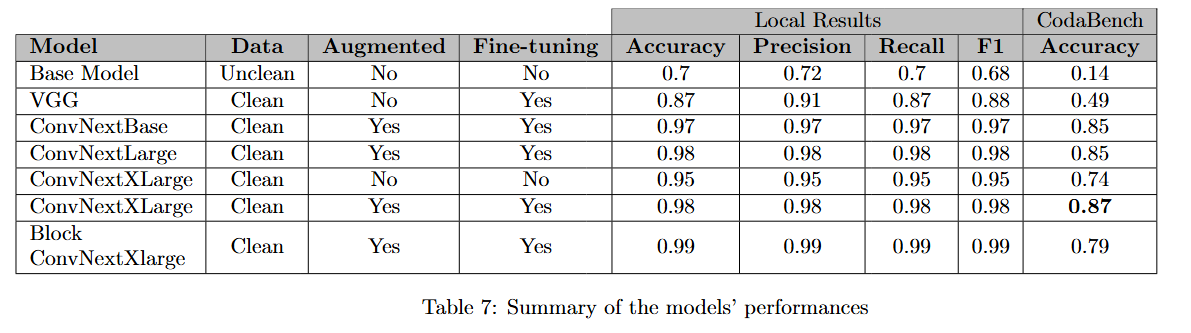
\includegraphics[width=\textwidth]{images/table.png} 
        \label{fig:Performance}
        % \captionof{figure}{text}
    \end{center}

    
    The approach effectively addressed challenges, achieving competitive performance across most cell types.
    It was proven that by carefully balancing class weights and fine-tuning key hyperparameters (such as the number of epochs, batch size, patience, ...) it was possible to achieve the same accuracy (85\%) with a ConvNext-Base model as with a ConvNext-Large model. Given that ConvNext-Base is significantly lighter and more computationally efficient, it presents a compelling alternative to ConvNext-Large, offering equivalent performance while requiring fewer resources. This underscores the effectiveness of optimization techniques in maximizing the efficiency of machine learning models.
    
    
    Future work could focus on generating synthetic data for rare classes or collecting additional images for easier and more precise training. It is also possible to experiment with lighter models for transfer learning and verify the change in performance.

    
    \section{Team contributions}
    \textbf{Angela} focused on data wrangling and implementing initial data augmentation techniques, including edge highlighting and developing the base model.
    \textbf{Pinar} worked on the ConvNext family models (Base, Large and XLarge models), applying fine-tuning to improve performance. 
    \textbf{Sergio} contributed by building and fine-tuning all VGG-based models, aiding comparative analysis. 
    \textbf{Matteo} tackled memory constraints through on-the-fly augmentation, optimizing the ConvNextXLarge model for better results.
    \textbf{All team members} collaborated on the project equally ensuring a balanced workload and a cohesive submission.

    
    \clearpage

% \FloatBarrier
% \begin{table*}[ht!]
%  \hskip-1.5cm
% \begin{tabular}{lccc|cccc|c|}
% \cline{5-9}
%                                                                                      & \multicolumn{1}{l}{}                                       & \multicolumn{1}{l}{}                                               & \multicolumn{1}{l|}{} & \multicolumn{4}{c|}{\cellcolor[HTML]{C0C0C0}Local Results}                                                                                                                                                      & \multicolumn{1}{l|}{\cellcolor[HTML]{C0C0C0}CodaBench} \\ \hline
% \rowcolor[HTML]{C0C0C0} 
% \multicolumn{1}{|l|}{\cellcolor[HTML]{C0C0C0}\textbf{Model}}                         & \multicolumn{1}{c|}{\cellcolor[HTML]{C0C0C0}\textbf{Data}} & \multicolumn{1}{c|}{\cellcolor[HTML]{C0C0C0}\textbf{Augmented}} & \textbf{Fine-tuning}  & \multicolumn{1}{c|}{\cellcolor[HTML]{C0C0C0}\textbf{Accuracy}} & \multicolumn{1}{c|}{\cellcolor[HTML]{C0C0C0}\textbf{Precision}} & \multicolumn{1}{c|}{\cellcolor[HTML]{C0C0C0}\textbf{Recall}} & \textbf{F1}   & \textbf{Accuracy}                                      \\ \hline
% \multicolumn{1}{|l|}{Base Model}                                                     & \multicolumn{1}{c|}{Unclean}                               & \multicolumn{1}{c|}{No}                                            & No                    & \multicolumn{1}{c|}{0.7}                                       & \multicolumn{1}{c|}{0.72}                                       & \multicolumn{1}{c|}{0.7}                                     & 0.68          & 0.14                                                   \\ \hline
% \multicolumn{1}{|l|}{VGG}                                                            & \multicolumn{1}{c|}{Clean}                                 & \multicolumn{1}{c|}{No}                                            & Yes                   & \multicolumn{1}{c|}{0.87}                                      & \multicolumn{1}{c|}{0.91}                                       & \multicolumn{1}{c|}{0.87}                                    & 0.88          & 0.49                                                   \\ \hline
% \multicolumn{1}{|l|}{ConvNextBase}                                                   & \multicolumn{1}{c|}{Clean}                                 & \multicolumn{1}{c|}{Yes}                                           & Yes                   & \multicolumn{1}{c|}{0.97}                                      & \multicolumn{1}{c|}{0.97}                                       & \multicolumn{1}{c|}{0.97}                                    & 0.97          & 0.85                                          \\ \hline
% \multicolumn{1}{|l|}{ConvNextLarge}                                                  & \multicolumn{1}{c|}{Clean}                                 & \multicolumn{1}{c|}{Yes}                                           & Yes                   & \multicolumn{1}{c|}{0.98}                             & \multicolumn{1}{c|}{0.98}                              & \multicolumn{1}{c|}{0.98}                           & 0.98 & 0.85                                          \\ \hline
% \multicolumn{1}{|l|}{ConvNextXLarge}                                                 & \multicolumn{1}{c|}{Clean}                                 & \multicolumn{1}{c|}{No}                                            & No                    & \multicolumn{1}{c|}{0.95}                                      & \multicolumn{1}{c|}{0.95}                                       & \multicolumn{1}{c|}{0.95}                                    & 0.95          & 0.74                                                   \\ \hline
% \multicolumn{1}{|l|}{ConvNextXLarge}                                                 & \multicolumn{1}{c|}{Clean}                                 & \multicolumn{1}{c|}{Yes}                                           & Yes                   & \multicolumn{1}{c|}{0.98}                                          & \multicolumn{1}{c|}{0.98}                                           & \multicolumn{1}{c|}{0.98}                                        & 0.98              & \textbf{0.87}                                                       \\ \hline
% \multicolumn{1}{|l|}{\begin{tabular}[c]{@{}l@{}}Block\\ ConvNextXlarge\end{tabular}} & \multicolumn{1}{c|}{Clean}                                 & \multicolumn{1}{c|}{Yes}                                           & Yes                   & \multicolumn{1}{c|}{0.99}                                          & \multicolumn{1}{c|}{0.99}                                           & \multicolumn{1}{c|}{0.99}                                        & 0.99              &    0.79                                                    \\ \hline
% \end{tabular}
%         \caption{Summary of the models' performances}
%         % \label{tab:Performance}
% \end{table*}




% \FloatBarrier        


        


    \bibliography{references}
    \bibliographystyle{abbrv}

    

    
    
    
    
    \end{multicols}
\end{document}